
\documentclass[a4paper, 10pt, twocolumn]{article}
\usepackage[top = 1.cm, left=1cm, right=1cm, bottom = 1.5cm]{geometry}
\usepackage[utf8]{inputenc}               
\usepackage[english]{babel}    
\usepackage{lipsum}
\usepackage{makecell}
\usepackage{graphicx}
\usepackage{enumitem}
\graphicspath{ {./images/} }

\begin{document}
\setlength{\parindent}{0pt}
\section{K-NN and /decision Trees}
Distances, $d(x^{(i)},x^{(q)})$ = \\
\begin{tabular}{| c | c | c | }
	\hline
	Manhattan & L1 & $\sum^{K}_{k=1}|x^{(i)}_{k} - x_{k}^{(q)}|$ \\ 
	\hline
	Euclidean & L2 & $\sqrt{\sum^{K}_{k=1}(x^{(i)}_{k} - x_{k}^{(q)})^2}$  \\  
	\hline
	Chebyshev & L$\infty$ & $\max^K_{k=1}|x^{(i)}_{k} - x_{k}^{(q)}|$  \\
	\hline 
\end{tabular} \\ \\ \\
Types = 
\begin{tabular}{ c c }
	Inverse & $\frac{1}{d(x^{(i)},x^{(q)})}$ \\ 
	Gaussian & $\frac{1}{\sqrt{2 \pi}}\exp(-\frac{d(x^{(i)},x^{(q)})^2}{2})$  \\     
\end{tabular} \\ \\ \\
Entropy = $H(X)$ =
\begin{tabular}{ c }
	$-\sum^K_k P(x_k) \log_2(P(x_k))$ \\
	$-\int_k f(x) \log_2(f(x))$
\end{tabular} \\ \\ \\
Information Gain = $\textrm{IG}(\textrm{dataset},\textrm{subsets})$\\ 
\begin{tabular} {c}
	$ = H(dataset) - \sum_{S \in \textrm{subsets}} \frac{|S|}{|\textrm{dataset}|}H(S)$ \\
	$|\textrm{dataset}| = \sum_{S \in \textrm{subsets}} |S|$
\end{tabular}
\section{Evaluation of Machine Learning Systems}
\textbf{Parameter Estimation}
\textit{Case 1:} Plenty of data available - Held-out test set
\begin{enumerate}[topsep=0pt,itemsep=-1ex,partopsep=1ex,parsep=1ex]
	\item Train algorithm on  \textbf{training set}
	\item Tune hyperparameters on  \textbf{validation set} 60:20:20 or 80:10:10 split
	\item Estimate generalisation performance using the  \textbf{test set}
\end{enumerate}
\textit{Case 2:} Limited data available - Cross-validation
\begin{enumerate}[topsep=0pt,itemsep=-1ex,partopsep=1ex,parsep=1ex]
	\item Separate dataset into  \textbf{k folds}
	\item Use 1 fold for testing and k-1 folds for  \textbf{training+validation}
	\item Repeat k times, using each fold as the  \textbf{test set}
	\item Estimate generalisation performance by \textbf{averaging results}
	across all the test folds
\end{enumerate}
Confusion Matrix \\ \\
\begin{tabular} {| c | c | c |}
	\hline
 & \thead{Class 1 \\ Predicted} & \thead{Class 2 \\ Predicted} \\
 \hline
 \thead{Class 1 \\ Actual} &  \thead{\bf TP \\ True Positive} & \thead{\bf FN \\False Negative} \\
 \hline
 \thead{Class 2 \\ Actual} &  \thead{\bf FP \\ False Positive} & \thead{\bf TN \\ True Negative} \\
 \hline
\end{tabular} \\\
\textbf{For Classification use:}
Accuracy = $\frac{TP + TN}{TP + TN + FP + FN}$ \\ 
Precision = $\frac{TP}{TP + FP}$ \\
Recall = $\frac{TP}{TP + FN}$ \\
F-measure = $F_1 = 2\frac{Precision*Recall}{Precision + Recall}$\\
\textbf{For regression use:}
MSE or RMSE
Sample Error: \\$error_s(h) = \frac{1}{N} \sum_{x \in S} \delta (f(x),h(x))$\\
Confidence interval: \\ $error_s(h) \pm Z_N \sqrt{\frac{error_s(h)*(1-error_s(h))}{n}}$
\section{Neural Networks}
Perceptron: \\
$\theta_i = \theta_i + \alpha(y-h(x))x_i$ \\
Classification: \\
\textbf{Binary:} Only two possible classes \\
\textbf{Multi-class:} More than one possible class but each class is distinct \\
\textbf{Multi-label:} Each input can belong to more than one class \\
Activation Functions: \\ 
\begin{tabular}{| c | c | c | c |}
	\hline
	\thead{Function} & $g(z)$ & $g'(z)$ & use\\
	\hline
	\thead{Threshold} & \thead{$1$: $W^Tx \geq 0 $ \\ $0:$ otherwise} & N/A & \thead{Perceptron} \\
	\hline
	\thead{Linear} & \thead{Duh} & \thead{Duh}  & \thead{Regression}\\
	\hline
	\thead{Sigmoid} & $\frac{1}{1 + e^{-x}}$ & $g(z)(1-g(z))$ & \thead{binary or \\ multi-label \\ classification}\\
	\hline
	\thead{Tanh} & $\frac{e^x  - e^{-x}}{e^x + e^{-x}}$ & $1-g(z)^2$ & \thead{binary or \\ multi-label \\ classification}\\
	\hline
	\thead{ReLU} & \thead{$0$ for $x \leq 0 $ \\ $x$ for $x>0$} & \thead{$0$ for $x \leq 0 $ \\ $1$ for $x>0$} &  \thead{Used in deep \\ layers and \\ regression} \\
	\hline
	\thead{Softmax} & $\frac{e^{Z_i}}{\sum_k e^{Z_k}}$ & $\frac{\delta L}{\delta z} = \frac{1}{N} (\hat y - y)$ & \thead{multi-class \\ classification}\\
	\hline
\end{tabular} \\ \\
Derivative of softmax only works for Cross entropy loss and N is the number of datapoints
Loss Functions: \\
\begin{tabular}{| c | c | c |}
	\hline 
	\thead{Name} & \thead{Definition} & \thead{Use} \\
	\hline
	\thead{MSE} & \thead{$\frac{1}{N} \sum^{N}_{i=1}(Y_i - \hat{Y}_i)^2$} & \thead{Regression} \\
	\hline
	\thead{Binary \\ cross-entropy} & \thead{$-\sum^{N}_{i=i}(y^{(i)}\log(\hat y^{(i)}) +$ \\ $(1-y^{(i)})\log (1-\hat y^{(i)}))$} & \thead{binary or \\ multi-label \\ classification} \\
	\hline
	\thead{Categorical \\  cross-entropy} & \thead{$-\sum^{N}_{i=1} \sum^{C}_{c=1}y_{c}^{(i)}\log(\hat y_{c}^{(i)})$} & \thead{multi-class \\ classification} \\
	\hline
\end{tabular} \\
Back Propagation:\\
$\frac{\delta \textrm{Loss}}{\delta W} = \frac{\delta \textrm{Loss}}{\delta Z} \cdot \frac{\delta Z}{\delta W}$ \\
$\frac{\delta \textrm{Loss}}{\delta b} = \frac{\delta \textrm{Loss}}{\delta Z} \cdot \frac{\delta Z}{\delta b}$ \\
$\frac{\delta \textrm{Loss}}{\delta X} = \frac{\delta \textrm{Loss}}{\delta Z} \cdot \frac{\delta Z}{\delta X}$ \\
$\frac{\delta \textrm{Loss}}{\delta X} = \frac{\delta \textrm{Loss}}{\delta Z} \cdot W^T$ \\
$\frac{\delta \textrm{Loss}}{\delta W} = X^T \cdot \frac{\delta \textrm{Loss}}{\delta Z}$ \\
$\frac{\delta \textrm{Loss}}{\delta b} = 1^T \cdot \frac{\delta \textrm{Loss}}{\delta Z}$ \\
$\frac{\delta \textrm{Loss}}{\delta Z} = \frac{\delta \textrm{Loss}}{\delta A} \circ g'(Z)$ \\
where $A = g(Z)$ \\ \\ Regularisation \\
$L1: J(\theta) = \textit{Loss}(y,\hat y) + \lambda \sum_w w^2$ \\
$w \leftarrow w - \alpha(\frac{\delta \textit{Loss}}{\delta w} + 2 \lambda w)$ \\
$L2: J(\theta) = \textit{Loss}(y,\hat y) + \lambda \sum_w |w|$ \\
$w \leftarrow w - \alpha(\frac{\delta \textit{Loss}}{\delta w} + 2 \sin w)$ \\
Dropout: drop $50\%$ of Activation \\ \\
Data normalisation\\
Min-Max: $X' = a + \frac{(X -X_{min})(b-a)}{X_{max}-X_{min}}$ \\
Standardization: $X' = \frac{X-\mu}{\sigma }$
\section{Unsupervised Learning} 
K-means \\
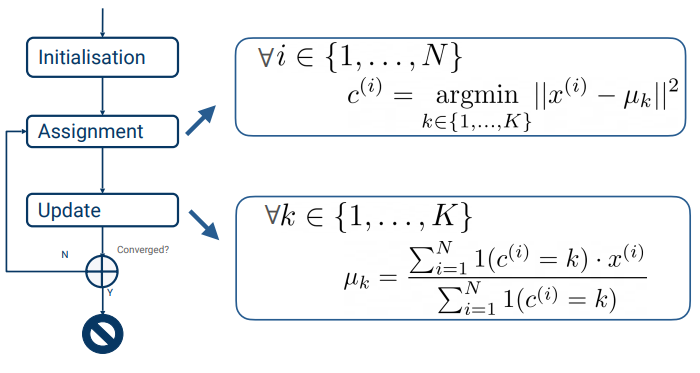
\includegraphics[scale=0.5]{k-means.png} \\
GMM-EM \\
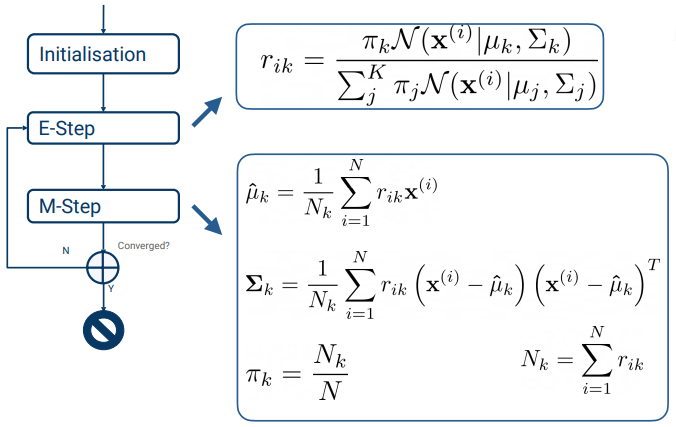
\includegraphics[scale=0.5]{GMM-EM.png} \\ \\
Mixture Models: \\$p(x) = \sum^K_{k=1} \pi_k p_k(x)$ \\
Gaussian Mixture models: \\$p(x|\theta) = \sum^K_{k=1} \pi_k \mathcal{N}(x|\mu_k, \sum_k)$ \\
\textbf{Negative Log likelihood} \\
$\mathcal{L} = -\sum^{N}_{i=1}\log P(x^{(i)}|\theta)$ \\
\textbf{Bayesian Information Criterion (BIC)}\\
$BIC_K = \mathcal{L}(K) + \frac{P_K}{2} \log(N) $ \\
\textbf{GMM-EM vs K-means:} \\
\begin{tabular}{| c | c |}
	\hline
	\thead{\textbf{K-means}} & \thead{\textbf{GMM-EM}} \\
	\hline
	\thead{Objective function: Minimize \\ average mean squared \\ distance} & \thead{Objective function: Maximize \\ log-likelihood} \\
	\hline
	\thead{EM-like algorithm \\ - Assignment: Assign \\ points to cluster \\ - Update: Optimise cluster } & \thead{EM algorithm \\ - E-step Compute posterior \\ probability of membership \\ - M-step: Optimise \\ parameters} \\
	\hline
	\thead{Performs hard assignment \\ during Assignment step} & \thead{Performs soft assignment \\ during E-step} \\
	\hline
	\thead{Assume spherical clusters \\ with equal probability for each \\ cluster} & \thead{Can be used for non-spherical \\clusters \\Can generate clusters with \\ different probabilities} \\
	\hline
\end{tabular}
\section{Evolutionary Algorithms}
genotype vs phenotype: gene representation vs what’s shown to environment genetic algorithm: intialize(
bitmaps for genomes), evaluate, select with selection operator(random roulette biased on fitness, tournament
by picking 1 from random 2), crossover using crossover operator(single-point crossover: swap a
prefix of parents for children), mutate using mutation operator(random bit flips)
elitism (GA): fix the top n\% of the population and ensure it survives (the fitness of the best individual
cannot decrease)
stopping criterion: individual with max fitness or fixed number of epochs or no improvement visible \\ \\

$\mu + \lambda$-ES algorithm: initialize $\mu + \lambda$ individuals (float array genotype), evaluate, select best $\mu$, generate
$\lambda$ offsprings by gaussian perturbations from random parents; usually $\frac{\lambda}{\mu} \approx 5$
main challenge is fixing $\sigma$2 for the gaussian distribution
one solution for fixing $\sigma$ is to add separate $\sigma$s for each gene and update them based on $\sigma$new = $\sigma \exp (\tau_0 \mathcal{N}(0, 1))$
where $\tau_0$ is the learning rate (usually $\tau_0 = \sqrt{n}$ where $n$ is the number of genes) \\ \\

novelty search: instead of optimizing for fitness optimize for novelty(using novelty archive composed of all
genotypes; average distance from kNN in novelty archive) behavioral descriptor(BD): defines the ”type
of solution” that is generated (not necessarily linked to task); several solutions can have same BD but
different fitnesses; evaluation AFTER selection \\ \\ 

Quality Diversity optimization: mix of novelty search and ES (interesting and high-performing solutions)
- highest performing solutions for each region of novelty archive; general pipeline: select population from
collection with selection operator, random mutation, evaluation, tenative addition to the collection
MAP-Elites - Multidimensional Archive of Phenotypic Elites: discretize the BD into a grid to try to fill it
with best solutions; hyperparameter is the size of cells
quantifying performance: the diversity of the container (archive size), the performance of the container
(max fitness), the convergence speed of the 2 points, QD score (sum of fitness of all solutions in the archive)
selector in MAP-Elites: usually uniform random
gradient descent can also be applied here using a critic or gradient estimation
\section{General}
Overfitting
\begin{itemize}[topsep=0pt,itemsep=-1ex,partopsep=1ex,parsep=1ex]
	\item high dimensionality $\rightarrow$  overfitting
	\item Stop for decision trees (Pruning, early stopping (max depth))
	\item General Solutions (more data, stop earlier and change complexity (use validation set to test))
	\item Neural networks (dropout/regularisation/normalisation)
\end{itemize}

\begin{tabular}{| c | c | c | c |}
	\hline
	\thead{Criteria} & \thead{Supervised \\ Learning} & \thead{Unsupervised \\ Learning} & \thead{Reinforcement \\ Learning} \\
	\hline
	\thead{Definition} & \thead{The machine \\learns by using \\labeled data} & \thead{The machine is \\ trained on \\unlabeled data\\ without any \\guidance} & \thead{An agent interacts \\ with its environment\\ by  performing actions \\ and  learning for \\ errors or rewards} \\
	\hline
	\thead{Types of \\ problems} & \thead{Regression and \\ classification} & \thead{Association and \\ clustering} & \thead{reward based} \\
	\hline
	\thead{Type of \\ data} & \thead{Labeled data} & \thead{Unlabeled data} & \thead{No predefined data} \\
	\hline 
	\thead{Training} & \thead{External \\ supervision} & \thead{no supervision} & \thead{no supervision} \\
	\hline
	\thead{Approach} & \thead{Maps the labeled \\inputs to the \\known outputs} & \thead{Understand patterns \\ and discovers the \\ outputs} & \thead {Follows the trial \\ and error method} \\
	\hline
\end{tabular}
\end{document}